% !TeX root = ./main.tex
\documentclass[letterpaper]{article}

\usepackage[spanish,es-tabla]{babel}
\usepackage[table,xcdraw]{xcolor}
\usepackage[nottoc]{tocbibind}
\usepackage{graphicx}
\usepackage{hyperref}
\usepackage{subfiles}
\usepackage{fancyhdr}
\usepackage{float}
\usepackage[left=3cm,right=3cm,top=3cm,bottom=4cm]{geometry}
\usepackage[acronym, toc, style=indexgroup]{glossaries}
\usepackage{hyperref}
\usepackage{multicol}
\usepackage{pdfpages}
\usepackage{listings}

\usepackage{xcolor}

\definecolor{codegreen}{rgb}{0,0.6,0}
\definecolor{codegray}{rgb}{0.5,0.5,0.5}
\definecolor{codepurple}{rgb}{0.58,0,0.82}
\definecolor{backcolour}{rgb}{0.95,0.95,0.92}

\lstdefinestyle{mystyle}{
    backgroundcolor=\color{backcolour},   
    commentstyle=\color{codegreen},
    keywordstyle=\color{magenta},
    numberstyle=\tiny\color{codegray},
    stringstyle=\color{codepurple},
    showstringspaces=false,
    commentstyle=\color{red},
    keywordstyle=\color{blue}basicstyle=\ttfamily\footnotesize,
    breakatwhitespace=false,         
    breaklines=true,                 
    captionpos=b,                    
    keepspaces=true,                 
    numbers=left,                    
    numbersep=5pt,                  
    showspaces=false,                
    showstringspaces=false,
    showtabs=false,                  
    tabsize=2
}

\lstset{style=mystyle}


\pagestyle{fancy}
\fancyfoot[R]{\thepage}
\fancyfoot[C]{
\includegraphics[width=0.1\textwidth]{inge_logo}}
\fancyhead[L]{\leftmark}
\fancyhead[R]{\rightmark}


\graphicspath{
  {img/}{images/}
}

\makeglossary{}
\documentclass[letterpaper]{article}

\usepackage[spanish,es-tabla]{babel}
\usepackage[table,xcdraw]{xcolor}
\usepackage[nottoc]{tocbibind}
\usepackage{graphicx}
\usepackage{hyperref}
\usepackage{subfiles}
\usepackage{fancyhdr}
\usepackage{float}
\usepackage[left=3cm,right=3cm,top=3cm,bottom=4cm]{geometry}
\usepackage[acronym, toc, style=indexgroup]{glossaries}
\usepackage{hyperref}
\usepackage{multicol}


\pagestyle{fancy}
\fancyhead[L]{\thepage}
\fancyfoot[C]{
\includegraphics[width=0.1\textwidth]{inge_logo}}



\graphicspath{
  {img/}{images/}
}

\makeglossary{}
\documentclass[letterpaper]{article}

\usepackage[spanish,es-tabla]{babel}
\usepackage[table,xcdraw]{xcolor}
\usepackage[nottoc]{tocbibind}
\usepackage{graphicx}
\usepackage{hyperref}
\usepackage{subfiles}
\usepackage{fancyhdr}
\usepackage{float}
\usepackage[left=3cm,right=3cm,top=3cm,bottom=4cm]{geometry}
\usepackage[acronym, toc, style=indexgroup]{glossaries}
\usepackage{hyperref}
\usepackage{multicol}


\pagestyle{fancy}
\fancyhead[L]{\thepage}
\fancyfoot[C]{
\includegraphics[width=0.1\textwidth]{inge_logo}}



\graphicspath{
  {img/}{images/}
}

\makeglossary{}
\documentclass[letterpaper]{article}

\usepackage[spanish,es-tabla]{babel}
\usepackage[table,xcdraw]{xcolor}
\usepackage[nottoc]{tocbibind}
\usepackage{graphicx}
\usepackage{hyperref}
\usepackage{subfiles}
\usepackage{fancyhdr}
\usepackage{float}
\usepackage[left=3cm,right=3cm,top=3cm,bottom=4cm]{geometry}
\usepackage[acronym, toc, style=indexgroup]{glossaries}
\usepackage{hyperref}
\usepackage{multicol}


\pagestyle{fancy}
\fancyhead[L]{\thepage}
\fancyfoot[C]{
\includegraphics[width=0.1\textwidth]{inge_logo}}



\graphicspath{
  {img/}{images/}
}

\makeglossary{}
\input{./main.tex.glo}

\begin{document}

\begin{titlepage}
  \centering
  
\includegraphics[width=0.3\textwidth]{unam_logo}\vfill{}
  {\scshape\Huge Facultad de Ingeniera\par}\vspace{0.5cm}
  {\scshape\Large Redes de Datos Seguras\par}\vfill
  {\huge \textbf{Proyecto 1}\\Planeación, optimización y
    rediseño de una red cableada}\vfill
  
  {\Large
    Alumnos\begin{itemize}
    \item Garrido Czacki Mario Horacio
    \item Romero Andrade Cristian
    \item Romero Andrade Vicente

    \end{itemize}
  }\vfill
  {\large Profesor: Ing.~Edgar Martinez Meza}\vfill
  
\includegraphics[width=0.1\textwidth]{inge_logo}
  
  
\end{titlepage}

\tableofcontents{}\newpage

\section{Resumen}\label{sec:resumen}

El \gls{cabesct}  ha  surgido  y  mejorado  con
el  pasar  del  tiempo  como  una opción de establecer
redes de área local LAN más estables, seguras y veloces
que han de solventar gran cantidad  de inconvenientes de
conexión,  intrusiones y tráfico lento,entre otros problemas
que deben enfrentar los diseñadores de red.

En este proyecto se plantea el cableado de la segunda planta
del Instituto de geografía, tratando de una excelente cotización
con excelente calidad-precio para el cableado, la instalación de
los equipos con sus configuraciones correspondientes.
tomando en cuenta el tiempo de vida
de la futura red. 

\section{Objetivos}\label{sec:obj}

\subsection{Objetivo General}\label{sec:objgen}

Elaborar la Planeación, optimización y rediseño de la red Cableada interna del
Instituto de Geografía de la UNAM.\ El diseño de la red abarcará aspectos físicos
y lógicos (\gls{cabesct} y direccionamiento lógico), así como la
aplicación de los conceptos estudiados en los tema 3 y 5 de la materia de Redes
de Datos Seguras.

\section{Escenario}\label{sec:esc}

La red que se implementará abarca el edificio Principal del Instituto del Instituto
de Geografía. Es necesario tener las siguientes consideraciones:
\begin{itemize}
\item El enlace de acometida principal deberá ser con tecnología de fibra
  óptica y se tomará desde el anillo de red UNAM, nota éste ya existe.
  
\item  En el edificio Principal existen dos Terrazas en la que no se puede realizar
el cableado, sin embargo se necesita conectividad.

\item También existen áreas donde no se puede realizar cableado pero se
  necesita conectividad. (Revisar en los planos)
  
\item  Los cuartos de telecomunicaciones el MDF y los IDF’s sólo pueden
instalarse en áreas permitidas, éstos deben estar conectados a través de
fibra óptica, entre cada uno de los IDFs y el MDF.\@

\item Los cubículos son ocupados por un investigador y sus becarios y las áreas
más grandes llamadas peceras albergan varios becarios. Considere el
número de nodos adecuado para cada área y las direcciones IP que se
van a requerir.

\item  En caso de que haya más de un área de trabajo por piso deberá aplicar
direccionamiento lógico VLSM y poner las IPs correspondientes a cada
área.
\end{itemize}

\newpage{}

\section{Desarrollo}\label{sec:ana}

\subfile{contenido/analisis}

\subsection{Estimaciones}\label{sec:sc}

\subfile{contenido/cotizacion}

\subsection{Propuesta}\label{sec:pro}

\subfile{contenido/subredes}

\newpage{}

\printglossary{}

\newpage{}

\listoftables
%\addcontentsline{toc}{chapter}{\listtablename}
\listoffigures


\end{document}


\begin{document}

\begin{titlepage}
  \centering
  
\includegraphics[width=0.3\textwidth]{unam_logo}\vfill{}
  {\scshape\Huge Facultad de Ingeniera\par}\vspace{0.5cm}
  {\scshape\Large Redes de Datos Seguras\par}\vfill
  {\huge \textbf{Proyecto 1}\\Planeación, optimización y
    rediseño de una red cableada}\vfill
  
  {\Large
    Alumnos\begin{itemize}
    \item Garrido Czacki Mario Horacio
    \item Romero Andrade Cristian
    \item Romero Andrade Vicente

    \end{itemize}
  }\vfill
  {\large Profesor: Ing.~Edgar Martinez Meza}\vfill
  
\includegraphics[width=0.1\textwidth]{inge_logo}
  
  
\end{titlepage}

\tableofcontents{}\newpage

\section{Resumen}\label{sec:resumen}

El \gls{cabesct}  ha  surgido  y  mejorado  con
el  pasar  del  tiempo  como  una opción de establecer
redes de área local LAN más estables, seguras y veloces
que han de solventar gran cantidad  de inconvenientes de
conexión,  intrusiones y tráfico lento,entre otros problemas
que deben enfrentar los diseñadores de red.

En este proyecto se plantea el cableado de la segunda planta
del Instituto de geografía, tratando de una excelente cotización
con excelente calidad-precio para el cableado, la instalación de
los equipos con sus configuraciones correspondientes.
tomando en cuenta el tiempo de vida
de la futura red. 

\section{Objetivos}\label{sec:obj}

\subsection{Objetivo General}\label{sec:objgen}

Elaborar la Planeación, optimización y rediseño de la red Cableada interna del
Instituto de Geografía de la UNAM.\ El diseño de la red abarcará aspectos físicos
y lógicos (\gls{cabesct} y direccionamiento lógico), así como la
aplicación de los conceptos estudiados en los tema 3 y 5 de la materia de Redes
de Datos Seguras.

\section{Escenario}\label{sec:esc}

La red que se implementará abarca el edificio Principal del Instituto del Instituto
de Geografía. Es necesario tener las siguientes consideraciones:
\begin{itemize}
\item El enlace de acometida principal deberá ser con tecnología de fibra
  óptica y se tomará desde el anillo de red UNAM, nota éste ya existe.
  
\item  En el edificio Principal existen dos Terrazas en la que no se puede realizar
el cableado, sin embargo se necesita conectividad.

\item También existen áreas donde no se puede realizar cableado pero se
  necesita conectividad. (Revisar en los planos)
  
\item  Los cuartos de telecomunicaciones el MDF y los IDF’s sólo pueden
instalarse en áreas permitidas, éstos deben estar conectados a través de
fibra óptica, entre cada uno de los IDFs y el MDF.\@

\item Los cubículos son ocupados por un investigador y sus becarios y las áreas
más grandes llamadas peceras albergan varios becarios. Considere el
número de nodos adecuado para cada área y las direcciones IP que se
van a requerir.

\item  En caso de que haya más de un área de trabajo por piso deberá aplicar
direccionamiento lógico VLSM y poner las IPs correspondientes a cada
área.
\end{itemize}

\newpage{}

\section{Desarrollo}\label{sec:ana}

\subfile{contenido/analisis}

\subsection{Estimaciones}\label{sec:sc}

\subfile{contenido/cotizacion}

\subsection{Propuesta}\label{sec:pro}

\subfile{contenido/subredes}

\newpage{}

\printglossary{}

\newpage{}

\listoftables
%\addcontentsline{toc}{chapter}{\listtablename}
\listoffigures


\end{document}


\begin{document}

\begin{titlepage}
  \centering
  
\includegraphics[width=0.3\textwidth]{unam_logo}\vfill{}
  {\scshape\Huge Facultad de Ingeniera\par}\vspace{0.5cm}
  {\scshape\Large Redes de Datos Seguras\par}\vfill
  {\huge \textbf{Proyecto 1}\\Planeación, optimización y
    rediseño de una red cableada}\vfill
  
  {\Large
    Alumnos\begin{itemize}
    \item Garrido Czacki Mario Horacio
    \item Romero Andrade Cristian
    \item Romero Andrade Vicente

    \end{itemize}
  }\vfill
  {\large Profesor: Ing.~Edgar Martinez Meza}\vfill
  
\includegraphics[width=0.1\textwidth]{inge_logo}
  
  
\end{titlepage}

\tableofcontents{}\newpage

\section{Resumen}\label{sec:resumen}

El \gls{cabesct}  ha  surgido  y  mejorado  con
el  pasar  del  tiempo  como  una opción de establecer
redes de área local LAN más estables, seguras y veloces
que han de solventar gran cantidad  de inconvenientes de
conexión,  intrusiones y tráfico lento,entre otros problemas
que deben enfrentar los diseñadores de red.

En este proyecto se plantea el cableado de la segunda planta
del Instituto de geografía, tratando de una excelente cotización
con excelente calidad-precio para el cableado, la instalación de
los equipos con sus configuraciones correspondientes.
tomando en cuenta el tiempo de vida
de la futura red. 

\section{Objetivos}\label{sec:obj}

\subsection{Objetivo General}\label{sec:objgen}

Elaborar la Planeación, optimización y rediseño de la red Cableada interna del
Instituto de Geografía de la UNAM.\ El diseño de la red abarcará aspectos físicos
y lógicos (\gls{cabesct} y direccionamiento lógico), así como la
aplicación de los conceptos estudiados en los tema 3 y 5 de la materia de Redes
de Datos Seguras.

\section{Escenario}\label{sec:esc}

La red que se implementará abarca el edificio Principal del Instituto del Instituto
de Geografía. Es necesario tener las siguientes consideraciones:
\begin{itemize}
\item El enlace de acometida principal deberá ser con tecnología de fibra
  óptica y se tomará desde el anillo de red UNAM, nota éste ya existe.
  
\item  En el edificio Principal existen dos Terrazas en la que no se puede realizar
el cableado, sin embargo se necesita conectividad.

\item También existen áreas donde no se puede realizar cableado pero se
  necesita conectividad. (Revisar en los planos)
  
\item  Los cuartos de telecomunicaciones el MDF y los IDF’s sólo pueden
instalarse en áreas permitidas, éstos deben estar conectados a través de
fibra óptica, entre cada uno de los IDFs y el MDF.\@

\item Los cubículos son ocupados por un investigador y sus becarios y las áreas
más grandes llamadas peceras albergan varios becarios. Considere el
número de nodos adecuado para cada área y las direcciones IP que se
van a requerir.

\item  En caso de que haya más de un área de trabajo por piso deberá aplicar
direccionamiento lógico VLSM y poner las IPs correspondientes a cada
área.
\end{itemize}

\newpage{}

\section{Desarrollo}\label{sec:ana}

\subfile{contenido/analisis}

\subsection{Estimaciones}\label{sec:sc}

\subfile{contenido/cotizacion}

\subsection{Propuesta}\label{sec:pro}

\subfile{contenido/subredes}

\newpage{}

\printglossary{}

\newpage{}

\listoftables
%\addcontentsline{toc}{chapter}{\listtablename}
\listoffigures


\end{document}


\begin{document}

\begin{titlepage}
  \centering
  
\includegraphics[width=0.3\textwidth]{unam_logo}\vfill{}
  {\scshape\Huge Facultad de Ingeniera\par}\vspace{0.5cm}
  {\scshape\Large Redes de Datos Seguras\par}\vfill
  {\huge \textbf{Proyecto 2 --- ORPHEUS}\\Monitoreo del tráfico a través del
servicio de SNMP graficado con MRTG}\vfill
  
  {\Large
    Alumnos\begin{itemize}
    \item Garrido Czacki Mario Horacio
    \item Romero Andrade Cristian
    \item Romero Andrade Vicente

    \end{itemize}
    \textbf{Equipo 3}
  }\vfill
  {\large Profesor: Ing.~Edgar Martinez Meza}\vfill
  
\includegraphics[width=0.1\textwidth]{inge_logo}
  
  
\end{titlepage}

\tableofcontents{}\newpage

\section{Resumen}\label{sec:resumen}

En el siguiente trabajo se implementa un sistema de
monitorización de red mediante el uso del protocolo \acrshort{snmp} y 
el software de monitoreo \acrshort{mrtg}. 
Con esto se busca obtener un seguimiento visual de equipos en una red y poder realizar
análisis de su comportamiento.

\section{Objetivos}\label{sec:obj}

\subsection{Objetivos Generales}\label{sec:objgen}
\begin{itemize}
\item Conocer el funcionamiento de los protocolos de acuerdo a sus capas
\item Utilizar una aplicacion real para la administracion y monitorizacion de una red
\item Tener una presentacion final de la informacion recopilada a travez de la red
\end{itemize}
\subsection{Objetivos Especificos}\label{sec:objgen}
\begin{itemize}
\item Implementar un servicio \acrshort{mrtg} que recopile los datos de una impresora o switch por medio de \acrshort{snmp}
\item Mostrar los datos tratados por el \acrshort{mrtg} en un servidor web seguro
\end{itemize}
\section{Desarrollo}\label{sec:objgen}
Lo primero a efectuar es la investigacion del funcionamiento de protocolo \acrshort{snmp} el cual tiene una historia
y sus casos de uso que lo hacen ideal para la monitorizacion de dispositivos de red.
\subsection{SNMP} % (fold)
Fue introducido en 1988 debido a la necesidad creciente de un estándar para
administrar dispositivos sobre redes IP.\@ Se trata de un protocolo de capa de aplicación
(capa 7, OSI) que facilita el intercambio de información de gestión entre dispositivos de
red.\\\\
Este protocolo es parte del conjunto de protocolos TCP/IP (Transmission
Control Protocol/Internet Protocol) y, por su amplia utilización en redes empresariales,
es considerado el estándar de facto en detrimento del protocolo CMIP (Common
Management Information Protocol) basado en el modelo OSI, más utilizado en las
grandes redes de las operadoras de telecomunicación. \acrshort{snmp} permite a los
administradores: gestionar el rendimiento, encontrar y solucionar problemas, y
planificar el crecimiento futuro de la red.\\\\
Si bien \acrshort{snmp} se diseñó, en un principio, con el propósito de hacer posible
supervisar de forma sencilla y resolver problemas en routers y bridges; con su
ampliación, este protocolo puede ser utilizado para supervisar y controlar: routers,
switches, bridges y hubs de la mayoría de fabricantes, además de servidores y
estaciones Windows y Unix, servidores de terminal, etc.\\\\
La información que se puede monitorizar son parámetros simples y
estandarizados para todos los routers y/o switches (independientemente del fabricante)
como por ejemplo la cantidad de tráfico de entrada y salida de una interfaz, el tiempo
que llevan encendidos, la carga de CPU, etc. Y parámetros más específicos
proporcionados por el fabricante del dispositivo, como puede ser la temperatura.\\\\
Se pueden resumir sus características en los siguientes puntos:
\begin{itemize}
  \item  Permite a los administradores gestionar el rendimiento de la red, buscar y
modificar la información de los dispositivos que la componen, encontrar y
diagnosticar problemas en la red, planificar su crecimiento y generar
informes sobre los nodos de la red.
  \item Es capaz de gestionar eficazmente dispositivos de diferentes fabricantes.

  \item Ofrece una simple combinación de solicitud-respuesta y un modo de
notificación activo, así como tiempo de espera y mecanismos de
retransmisión.

  \item Contiene pocos tipos de paquetes con un formato sencillo, facilitando su
resolución e implementación.
  \item Dispone de mecanismos de autenticación y privacidad como medidas de
  \item Emplea UDP en el puerto 161 para el envio y recepcion de solicitudes
  \item Empleta UDP en el puerto 162 para la recepcion de los agentes ``traps''
  \item Existen 3 versiones del protocolo
  \begin{itemize}
    \item SNMPv1 --- version inicial del protocolo estandarizado
    \item SNMPv2-c --- Solventa problemas de seguridad y sobrecargas en transferencias de datos.
    \item SNMPv3 --- Añade esquemas de autenticación y encriptación
  \end{itemize}
\end{itemize}
\subsection{SMI y MIB}\label{sub:objgen} % (fold)
La SMI (Structure of Managemet Information) se encarga de definir un esquema
de nombres únicos para cada uno de los objetos administrados y su comportamiento
(denominado OID). El agente posee una lista de los objetos que son supervisados, como
puede ser el estado operacional de la interfaz de un router (“up” o “down”).\\\\
La MIB (Management Information Base) se puede considerar como una base de
datos que almacena información (los OIDs con su descripción) de los dispositivos
administrados. Al igual que el Agente reside en cada uno de los dispositivos
gestionados. Las MIBs contienen objetos que representan parámetros o variables de los
equipos gestionados y se ordenan de forma jerárquica siguiendo un esquema de árbol.
Estas colecciones de objetos relacionados, definidos como módulos de MIB.\@ Estos
módulos están escritos en un lenguaje especial, definido en el estándar de Internet STD
58, y en los RFCs de Internet 2578, 2579 y 2580.\\\\
Cada elemento del árbol MIB se identifica por un OID (Object Identifier)
numérico o de texto. La lista completa de los objetos y su definición
correspondiente está definida en el RFC 1212.\\\\
% subsectionSMI y MIB (end)
% subsectionSNMP (end)
\subsection{MRTG}\label{sub:MRTG}% (fold)
Se trata de una herramienta para monitorizar diversos parámetros de red y
generar páginas HTML que contienen imágenes (con formato PNG) que proporcionan
una representación gráfica en vivo de los datos que obtiene del protocolo \acrshort{snmp} o de
scripts.\\\\
Entre las características más importantes de \acrshort{mrtg} tenemos las siguientes:
\begin{itemize}
  \item Está escrito en Perl.
  \item  Utiliza una aplicación \acrshort{snmp} portátil escrito completamente en Perl, por lo
que no hay necesidad de instalar ningún paquete externo \acrshort{snmp}.\@
  \item  Las interfaces de routers pueden ser fácilmente identificadas por su dirección
IP, la descripción y la dirección Ethernet además de la interfaz de serie
normal.
  \item Los gráficos son generados directamente en formato PNG
  \item El aspecto de las páginas web producidas por \acrshort{mrtg} así como la
configuración de este son altamente configurables.
\end{itemize}
\acrshort{mrtg} consiste en un script de Perl que utiliza el protocolo \acrshort{snmp} para
controlar cualquier variable que se elija, y un rápido programa en C que registra el
tráfico de datos y crea los gráficos para representarlos. Estos gráficos se incrustan
entonces en páginas web.
% subsection MRTG (end)
\begin{figure}[H]
  \centering
  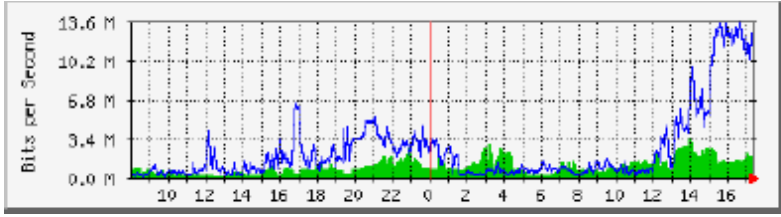
\includegraphics[width=\textwidth]{images/MRTG.png}
  \caption{Grafica generada con MRTG.}\label{fig:mrtg}
\end{figure}
\section{Configuracion}\label{sec:objgen}
Para esta configuracion se hizo uso de un equipo con las siguientes caracteristicas:
\begin{itemize}
  \item Computadora conectada via inalambrica a internet
  \item Archlinux como sistema operativo
  \item Servidor Nginx configurado con un dominio
\end{itemize}
Los pasos seguidos son los siguientes:
\begin{itemize}
  \item Instalar \acrshort{mrtg}\\\begin{lstlisting}
pacman -S mrtg
\end{lstlisting}
  \item Crear el usuario mrtg \\\begin{lstlisting}
  useradd -d /srv/http/mrtg mrtg
\end{lstlisting}
  \item Crear el directorio home del usuario y darle permisos\\
  \begin{lstlisting}
    mkdir /srv/http/mrtg
    chown mrtg:mrtg /srv/http/mrtg
  \end{lstlisting}
  \item asignar el dominio y su configuracion a nginx
  \begin{lstlisting}
    cp /configs/mrtg.somch.org /etc/nginx/available-site/
    ln -s /etc/nginx/available-sites/mrtg.somch.org /etc/nginx/enabled-sites/mrtg.somch.org
    systemctl reload nginx
  \end{lstlisting}
  \item Crear el directorio que albergara los archivos PNG y el index
  \begin{lstlisting}
    mkdir /srv/http/mrtg/html
  \end{lstlisting}
  \item Crear el archivo de configuracion mrtg
  \begin{lstlisting}
    cfgmaker --output=/srv/http/mrtg/mrtg.cfg --ifref=name --ifref=descr --global "WorkDir: /srv/http/mrtg" igg@132.247.103.251
  \end{lstlisting}
  \item Añaidr los parametros extra al archivo mrtg.cfg generado
  \begin{lstlisting}
    ### Global configuration  ###
    LoadMIBs: /usr/share/snmp/mibs/UCD-SNMP-MIB.txt
    EnableIPv6: no
    HtmlDir: /srv/http/mrtg/html
    ImageDir: /srv/http/mrtg/html
    LogDir: /srv/http/mrtg
    ThreshDir: /srv/http/mrtg
    RunAsDaemon: Yes
    Interval: 5
    Refresh: 60
  \end{lstlisting}
  \begin{enumerate}
    \item Corresponde a la base de datos gestionada MIB que contiene los parametros de los dispositivos compatibles
    \item Deshabilita el IPv6
    \item La ruta de los archivos html
    \item La ruta de las imagnes PNG
    \item La ruta de los archivos log
    \item El folder thresh
    \item Correr como demonio
    \item Intervalo en minutos del demonio, 5 minutos.
    \item Intervalo de refresco de archivos html.
  \end{enumerate}
  \item Una vez creado el archivo de configuracion ir al directorio /srv/http/mrtg y crear el index
  \begin{lstlisting}
    cd /srv/http/mrtg
    indexmaker ./mrtg.cfg > index.html
  \end{lstlisting}
  \item Crear el servicio que demonizara el servicio \acrshort{mrtg} que obtendra los datos
  \begin{lstlisting}
    cp configs/mrtg.service /usr/lib/systemd/system
    systemctl enable mrtg
    systemctl start mrtg
  \end{lstlisting}
  \item Abrir el dominio en el navegador y observar los resultados
\end{itemize}
\subsection{Archivos de configuracion usados}\label{sub:Archivos de configuracion usados} %fold
Archivo de la configuracion del subdominio de nginx
\lstinputlisting{configs/mrtg.somch.org}
Script que ejecuta el demonio
\lstinputlisting[language=bash]{configs/mrtg.sh}
Archivo de configuracion systemd
\lstinputlisting{configs/mrtg.service}

% subsection Archivos de configuracion usados (end)
\newpage{}

\printglossary[type=\acronymtype]

\printglossary{}

\end{document}
